%\sub
\seccion{Variedad Topol\'ogica}
\label{s:WL:VariedadToplogica}

Nuestra experiencia cotidiana de percibir  que estamos inmersos en un espacio de
3 dimensiones, en el cual  podemos medir \'angulos y determinar distancias entre
dos puntos, ha  hecho que usemos estas caracteristicas  de nuestro habitat, como
motivaci\'on de  la defici\'on de ciertas estructuras  matem\'aticas en espacios
abstractos.

En primer lugar, con la noci\'on de una variedad topol\'ogica buscaremos simular
en  un conjunto  cualquiera, la  noci\'on  de cercan\'ia  y dimensionalidad  que
tenemos en $\Rset^n$.

\begin{definicion}[Variedad topol\'ogica $n$-dimensional]
  Una  {\it Variedad  topol\'ogica $n$-dimensional}  es un  espacio topol\'ogico
  $\M$ tal que es {\it localmente eucl\'ideo}, es decir que para cada $x \in \M$
  existe  un  entorno  abierto $U$  de  $x$,  homeomorfo  a  un abierto  $V$  de
  $\Rset^n$: \ $\phi: U \subseteq \M \rightarrow \Rset^n$ \
  %
  % \[
  % \phi: U \subseteq \M \rightarrow \Rset^n
  % \]
  %
  tal que \ $\phi:U \rightarrow V$ \
  % \[
  % \phi:U \rightarrow V
  % \]
  y  $\phi$ es  un homeomorfismo.  Tambi\'en  pediremos que  $\M$, como  espacio
  topol\'ogico, sea un espacio Hausdorff.
\end{definicion}
%
A los pares  $(U,\phi)$ se los denominan {\it cartas sobre  $\M$}. Se supone que
la  colecci\'on de  todas las  cartas cubren  completamente a  $\M$.  Las cartas
permiten asignar {\it coordenadas} a $\M$:
%
\[
\mbox{Si}  \quad  p \in  U  \subseteq \M  \quad  \mbox{entonces}  \quad \phi:  p
\rightarrow (p_1 , \ldots , p_n) \in \Rset^n
\]

\begin{figure}[h!]
  \centerline{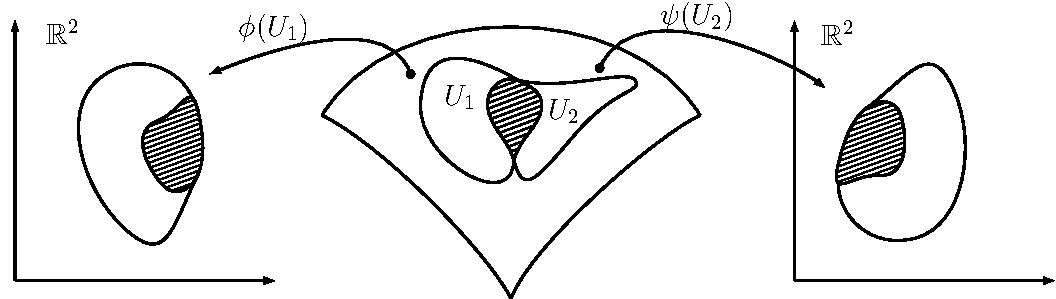
\includegraphics[width=13cm]{figura1.pdf}}          \leyenda{Cartas
    coordenadas usadas en la definici\'on de una variedad topol\'ogica.}
\end{figure}

A  la colecci\'on  de n\'umeros  reales $(p_1  , \ldots  , p_n)$  se  llaman las
coordenadas  de  $p$  de  acuerdo  a  la carta  $(U,\phi)$.   La  existencia  de
coordenadas, es el aspecto fundamental por el que el concepto de variedad es tan
\'util en f\'isica.

Podr\'ia suceder que un mismo punto $p$ pertenezca a m\'as de una carta, digamos
$(U_1,\phi_1)$  y  $(U_2,\psi_2)$.  En  ese  caso  hablaremos  de un  cambio  de
coordenadas:
%
\begin{equation}\label{cc}
\psi \circ \phi^{-1}: \phi(U_1 \cap U_2) \rightarrow \psi(U_1 \cap U_2)
\end{equation}
%
Si denotamos por $(p_1 , \ldots  , p_n)$ a las coordenadas correspondientes a la
carta  $(U_1,\phi_1)$  y  por  $(\tilde{p}_1  , \ldots  ,  \tilde{p}_n)$  a  las
correspondientes a la carta  $(U_2,\psi_2)$, entonces las funciones $\tilde{p}_i
= \tilde{p}_i(p_1 ,  \ldots , p_n)$ son funciones continuas, y  dan el cambio de
coordenadas. Estas funciones son invertibles con inversa continua.

Ejemplos de variedades topol\'ogicas son:
%
\begin{itemize}
\item $\Rset^n$. En este caso hay  una carta coordenada global que cubre toda la
  variedad y donde el homeomorfismo es la identidad.
%
\item $\Sset^n$, la esfera de dimensi\'on $n$. Ella est\'a definida como el conjunto:
  \[
  \Sset^n = \left\{  (x_1 , \ldots ,  x_{n+1}), \: x_i \in \Rset:  \quad x_1^2 +
    \cdots + x_{n+1}^2 = 1 \right\}
  % \text{ tales que }
  \]
\end{itemize}
%
\noindent  Se debe observar  que al  definir $\Sset^n$  no estamos  pensando que
est\'a inmersa  en $\Rset^n$. En este  caso podemos usar  las siguientes cartas:
$(U_N,  \phi_N)$ y $(U_S,\phi_S)$,  donde $U_N  = \Sset^n-\{  (0,0,\ldots,1) \},
\quad U_S = \Sset^n -{(1,0,\ldots,0)}$ y los mapas
%
\[
\phi_N:  U_N  \rightarrow  \Rset^n  /  (\phi_N(x_1  ,  \ldots  ,  n_{n+1}))_i  =
\frac{x_i}{1-x_{n+1}}
\]
%
y
%
\[
\phi_S:  U_S  \rightarrow  \Rset^n  /  (\phi_N(x_1  ,  \ldots  ,  n_{n+1}))_i  =
\frac{x_i}{1+x_{n+1}}
\]
%
Ambos mapas son homeomorfismos.  Observemos  que $\phi_N(x_1 , \ldots , x_{n+1})
= (t x_1 , \ldots , t x_n)$ y  $\phi_S(x_1 , \ldots , x_{n+1}) = (u x_1 , \ldots
,  u  x_n)$   con  $t  =  \frac{1}{1-x_{n+1}}$  y   $u  =  \frac{1}{1+x_{n+1}}$,
respectivamente.  Es directo verificar la  inyectividad pues si $(t x_1 , \ldots
, t x_n) = (t  y_1 , \ldots , t y_n) \Rightarrow x_i =  y_i \quad \forall \: i$.
Entonces  los puntos  $x$  e $y$  son  id\'enticos.  Para  ver la  suryectividad
consideremos el punto  $y = (y_1 , \ldots  , y_n) \in \Rset^n$. Si  tomamos $x =
\left( t^{-1}  y_1 ,  \ldots , t^{-1}  y_n ,  y_{n+1} \right)$ con  $t \ne  0$ e
$y_{n+1} =  t \sqrt{1-(t^{-1}  y_1)^2 - \cdots  - \left( t^{-1}  y_n \right)^2}$
vemos que para cada $y \in \Rset^n$ existe un $x \in \Sset^n$ tal que $\phi(x) =
y$.   Usando las  expresiones  expl\'citas  de $\phi_N$  y  $\phi_S$ es  directo
verificar que se trata de funciones continuas.

{\bf Nota}:  Hay propiedades de las  variedades topol\'ogicas que  no tienen que
ver con sus  caracter\'isticas locales, las que hemos dicho  son similares a las
de  $\Rset^n$,  sino con  sus  propiedades  globales.   Por ejemplo  una  esfera
$2$-dimensional es  homeomorfa a  la superficie de  una pelota de  futbol, a\'un
cuando pensemos en una pelota de futbol verdadera, la cual es una colecci\'on de
parches hexagonales  o pentagonales,  unidos unos con  otros. Ambos  objetos, la
esfera  y la pelota  de futbol,  son objetos  compactos, cerrados  y simplemente
conexos.   Sin  embargo   un  toro  y  una  esfera   no  comparten  todas  estas
caracter\'isticas: un toro  es cerrado, compacto pero no  simplemente conexo, es
decir no  todo lazo sobre  \'el puede contraerse  continuamente a un  punto. Por
ello diremos que un toro y una esfera son localmente homeomorfos, pero no lo son
globalmente. Este tipo de situaciones  ha llevado a introducir cantidades que de
alguna  manera   caractericen  a  las  propiedades  globales   de  una  variedad
topol\'ogicas. Un ejemplo muy conocido  es la caracter\'istica de Euler. Para un
poliedro de  tres dimensiones la  caracteristica de Euler $\Xi$  est\'a definida
por
%
\[
\Xi = V - A + C
\]
%
donde  $V, A$ y  $C$ son  el n\'umero  de vertices,  de aristas  y de  caras del
poliedro, respectivamente. Para un cubo,  por ejemplo, $\Xi = 2$. Supongamos que
el cubo est\'a hecho en un  material el\'astico, apoyado sobre un armaz\'on (las
aristas) de metal. Si inflamos ese cubo, obtenemos una esfera. Matem\'aticamente
eso significa que el cubo y la efera son globalmente homeomorfos entre si, y por
lo  tanto topol\'ogicamente  equivalentes. Es  posible extender  el  concepto de
caracter\'istica  de Euler  a la  superficie  de una  esfera, a  trav\'es de  la
triangularizaci\'on de  la superficie esf\'erica,  es decir cubriendo  la esfera
por tri\'angulos.  En  ese caso la caracter\'istica de Euler  se calcula como el
n\'umero  de tri\'angulos  menos el  n\'umero de  aristas m\'as  el  n\'umero de
v\'ertices. Haci\'endo  ese c\'alculo  para la esfera  resulta el valor  $2$. Lo
mismo sucede con cualquier otro poliedro que se pueda deformarse continuamente a
una  esfera.  Hay maneras  de  definir la  caracter\'istica  de  Euler para  una
variedad topol\'ogica  arbitraria y esa cantidad es  un invariante topol\'ogico,
es decir  una cantidad que no  cambia entre variedades  homeom\'orficos. Para un
toro la caracter\'istica de Euler vale $0$.
